\documentclass[10pt]{article}
%\usepackage{url}
%\usepackage{algorithmic}
\usepackage[margin=1in]{geometry}
\usepackage{datetime}
\usepackage[margin=2em, font=footnotesize]{caption}
\usepackage{graphicx}
\usepackage{mathpazo} % use palatino
\usepackage[scaled]{helvet} % helvetica
\usepackage{microtype}
\usepackage{amsmath}
\usepackage{subfigure}
\usepackage{listings}
\usepackage{wrapfig}
\usepackage{ amssymb }
% Letterspacing macros
\newcommand{\spacecaps}[1]{\textls[200]{\MakeUppercase{#1}}}
\newcommand{\spacesc}[1]{\textls[50]{\textsc{\MakeLowercase{#1}}}}
\lstdefinestyle{myCustomMatlabStyle}{
  language=Matlab,
  stepnumber=1,
  numbersep=10pt,
  tabsize=4,
  showspaces=false,
  showstringspaces=false
}
\lstset{basicstyle=\footnotesize,style=myCustomMatlabStyle}
\title{\flushleft2.4 Sensitivity of Optimisation Algorithms to Initialisation\\ }
\date{}
\usepackage{dsfont}
\usepackage{varwidth}
\usepackage{float}
\usepackage{bm}

\begin{document}
5\hfill\framebox{\parbox[t][5 true cm][c]{11 true cm}
{\hfil Space for project label}}
\section*{\LARGE{2.4 Sensitivity of Optimisation Algorithms to Initialisation}}
\section*{Gradient Descent}
  \[f_{\theta}(x):[-1,1]\rightarrow\mathds{R}\qquad f_{\theta}(x)=(x^2-\frac{3}{4})^2-x\cos{\theta}\qquad \theta\in(0,\pi)\]
\subsection*{Question 1}
We differentiate $f$ with respect to $x$ to get
\[\frac{df}{dx}=4x(x^2-\frac{3}{4})-\cos{\theta}\]
Setting \(\frac{df}{dx}=0\) , we get
\begin{align*}
4x^3-3x &= \cos{\theta}\\
\intertext{then by using the triple angle rule for cosine ($\cos{3\theta}=4\cos^3{\theta}-3\cos{\theta}$), we obtain}
x &= \cos{\frac{\theta+2k\pi}{3}}\qquad k\in\mathds{Z}
\end{align*}
There exist three unique values of $x$ for the above equation, namely $x=\cos{\frac{\theta}{3}}$, $x=\cos{\frac{\theta+2\pi}{3}}$ and $x=\cos{\frac{\theta+4\pi}{3}}$. And these are the three stationary points of $f_{\theta}(x)$.\\
We differentiate $\frac{df}{dx}$ with respect to x again to get
\[\frac{d^2f}{dx^2}=12x^2-3\]
thus if $|x|<\frac{1}{2}$, $\frac{d^2f}{dx^2}<0$, the stationary point is a maximum; if $|x|=\frac{1}{2}$, $\frac{d^2f}{dx^2}=0$, the stationary point is a saddle point; and if $|x|>\frac{1}{2}$, $\frac{d^2f}{dx^2}>0$, the stationary point is a minimum.\\
For $\theta\in(0,\pi)$, we note $\cos{\frac{\theta}{3}}\in(\frac{1}{2},1),\quad\cos{\frac{\theta+2\pi}{3}}\in(\frac{-1}{2},-1)\quad\text{and}\quad\cos{\frac{\theta+4\pi}{3}}\in(\frac{-1}{2},\frac{1}{2})$.\\
Therefore, $x=\cos{\frac{\theta}{3}}$ is a local minimum;\\
$x=\cos{\frac{\theta+2\pi}{3}}$ is a local minimum;\\
$x=\cos{\frac{\theta+4\pi}{3}}$ is a local maximum.

\subsection*{Question 2}
The code used to produce the table below is attached in the programs section under the title \emph{'i) q2\textunderscore gradient\textunderscore descent.m'}\\
\begin{tabular}{ll}
\hline
initial point $x_0$ & outcome \\ 
\hline 
-1 & -0.64279 \\ 
-0.6 & -0.64279 \\ 
-0.4 & -0.64279 \\ 
-0.38 & -0.64279 \\ 
-0.36 & -0.64279 \\ 
-0.34 & 0.98481 \\ 
-0.32 & 0.98481 \\ 
-0.1 & 0.98481 \\ 
0.2 & 0.98481 \\ 
0.6 & 0.98481 \\ 
1 & 0.98481 \\ 
\hline 
\end{tabular}\\\\
We observe the algorithm converging to -0.64279 for all initial points ranging from -1 to -0.36; and the algorithm converging to 0.98481 for all initial points ranging from -0.34 to 1.\\
This suggests that there are two local minimums around x=-0.64279 and x=0.98481; and a local maximum between -0.34 and -0.36.\\
Which are accurate if we compare them to the analytic solutions of the stationary points of the function $f_{\theta}(x)$ with $\theta=\frac{\pi}{6}$, which has its local minimums at $x=\cos{\frac{\pi}{18}}=0.98481$, $x=\cos{\frac{13\pi}{18}}=-0.64279$; and its local maximum $x=\cos{\frac{25\pi}{18}}=-0.34202$.\\
So the outcomes suggest the gradient descent algorithm worked desirably to find the minimisers.

\section*{The Monte Carlo Method}
\(\nu=\bm{E}[g(X)];\qquad \{X^i\}_{i=1}^N \sim X\text{ i.i.d.};\qquad \text{estimator } \hat{\nu}_N\triangleq\frac{1}{N}\sum_{i=1}^{N}g(X^i)\)
\subsection*{Question 3}
\begin{flalign*}
\bm{E}[\hat{\nu}_N]&=\bm{E}[\frac{1}{N}\sum_{i=1}^{N}g(X^i)]&\\
&=\frac{1}{N}\sum_{i=1}^N\bm{E}[g(X^i)]\\
&=\frac{1}{N}\bm{E}[\sum_{i=1}^N g(X^i)]\\
\intertext{As $\{X^i\}_{i=1}^N \sim X\text{ i.i.d.}$ implies $g(X^i)\sim g(X)\text{ i.i.d.}$}
&=\frac{1}{N}\times N\times \bm{E}[g(X)]=\frac{N}{N}\nu=\underline{\nu}
\end{flalign*}
Therefore, the estimator $\hat{\nu}_N$ is unbiased.\\
Assuming $\bm{Var}(g(X))<\infty$,
\begin{flalign*}
\bm{Var}(\hat{\nu}_N)&=\bm{Var}[\frac{1}{N}\sum_{i=1}^{N}g(X^i)]&\\
&=\frac{1}{N^2}\sum_{i=1}^N\bm{Var}[g(X^i)]\qquad\qquad\text{(As $\{X^i\}_{i=1}^N \sim X\text{ i.i.d.}$ implies $g(X^i)\sim g(X)\text{ i.i.d.}$)}\\
&=\underline{\frac{1}{N}\bm{Var}[g(X)]}
\end{flalign*}

\subsection*{Question 4}
The code used to produce the tables below is attached in the programs section under the title \emph{'ii) q4\textunderscore monte\textunderscore carlo\textunderscore gradient\textunderscore descent.m'}\\\\
\begin{tabular}{lll}
k & estimate of $\mu^h$ & estimate of $\bm{Var}(X^h_ {Th^{-1}})$ \\ 
\hline 
0 & 0.34503 & 0.65327 \\ 
1 & 0.34397 & 0.65372 \\ 
2 & 0.34422 & 0.65362 \\ 
3 & 0.34289 & 0.65419 \\ 
4 & 0.34137 & 0.65484 \\ 
5 & 0.34288 & 0.65421 \\ 
6 & 0.35181 & 0.65034 \\ 
7 & 0.33997 & 0.6555 \\ 
8 & 0.33445 & 0.65788 \\ 
9 & 0.32383 & 0.66228 \\ 
10 & 0.34998 & 0.65175 \\ 
\hline 
\end{tabular}\\\\
We observe from the table that the value of $\mu^h$ oscillates frequently in the 0.34-0.35 region as k increases. There is no clear trend of the sequence converging to a limit or a decrease in the size of the difference between each iteration of $\mu^h$ as $h$ decreases, which is due to the decrease in the number of samples used for small $h$. \\
The estimates also suggests a small increase in the variance of $\bm{Var}(X^h_ {Th^{-1}})$ as h gets smaller, but the amount of increase also gets smaller as h gets smaller, which should converges as $h\to0^ +$. 

\subsection*{Question 5}
\(\bm{MSE}(T;\tau)\triangleq\bm{E}[(T-\tau)^2]\)
\begin{flalign*}
\bm{MSE}(T;\tau)&=\bm{E}[(T-\tau)(T-\tau)]&\\
&=\bm{E}[T^2-2T\tau+\tau^2]\\
&=\bm{E}[T^2]-2\tau\bm{E}[T]+\tau^2\qquad\qquad(\bm{Var}(T)=\bm{E}[T^2]-\bm{E}[T]^2)\\
&=\bm{Var}(T)+[\bm{E}[T]^2-t\tau\bm{E}[T]+\tau^2]=\underline{(\bm{E}[T]-\tau)^2+\bm{Var}(T)}
\end{flalign*}\\
Facts given:\\
1. the bias of the approximation $\mu^h$ is bounded as $|\mu^h-\mu|\leq A_1h$,\\
2. the variance of $X^h_{Th^{-1}}$ is bounded as $\bm{Var}(X^h_{Th^{-1})}\leq A_2$, and\\
3. for $t\in\{0,1,\dots\}$, the cost of generating a sample of $X_t^h$ satisfies \textbf{Cost}$(X^h_t)=A_3t$.
\subsection*{Question 6}
\(\hat{\mu}_N^h\triangleq\frac{1}{N}\sum_{i=1}^NY^i\qquad \{Y^i\}^N_{i=1}\sim X^h_{Th^{-1}}\text{ i.i.d. \qquad $h,N$ fixed}\)\\
\begin{flalign*}
\bm{MSE}(\hat{\mu}_N^h,\mu)&=(\bm{E}[\hat{\mu}_N^h]-\mu)^2+\bm{Var}(\hat{\mu}_N^h)&\\
&=(\bm{E}[X^h_{Th^{-1}}]-\mu)^2+\frac{1}{N}\bm{Var}(X^h_{Th^{-1}})\qquad\qquad\text{(using equations obtained in Question 3)}\\
&=(\mu^h-\mu)^2+\frac{1}{N}\bm{Var}(X^h_{Th^{-1}})\qquad\qquad\text{(using facts 1 and 2)}\\
&\leq A_1^2h^2+\frac{A_2}{N}\\
\intertext{If we choose some $(N,h)$ such that $N\times\frac{A_3T}{h}=C$, then $N=\frac{Ch}{A_3T}$ and}
\bm{MSE}(\hat{\mu}_N^h,\mu)&\leq A_1^2h^2+\frac{A_2A_3T}{Ch}
\end{flalign*}
to find h which minimises the upper bound we differentiate the above expression for the upper bound and equate it to 0:
\begin{flalign*}
&2hA_1^2-\frac{A_2A_3T}{Ch^2}=0&\\
&h=\sqrt[3]{\frac{A_2A_3T}{2CA_1^2}}
\end{flalign*}
Therefore, by writing $h$ as $k\times C^{-1/3}$, the optimal MSE's upper bound can be written as \[\bm{MSE}(\hat{\mu}_N^h,\mu)\leq A_1^2k^2C^{-2/3}+A_2A_3Tk^{-1}C^{-2/3}\]
\[=C^{-2/3}(A_1^2k^2+A_2A_3Tk^{-1})\]
Therefore, the optimal MSE $\propto C^{-2/3}$.\medskip

\section*{Multi-Level Monte Carlo}
Extra facts given:\\
4. If two sequences of gradient descent iterates have the same initial point $X_0\sim Uniform([-1,1])$, then $\bm{Var}(X^h_{Th_l^{-1}}-X^{h_{l-1}}_{Th_{l-1}^{-1}})\leq A_4h^2$.
\subsection*{Question 7}
\(\mu=\sum_{l\geq0}\bm{E}[Y_l]\qquad\) with \(\quad Y_0=X^{h_0}_{Th_0^{-1}}\quad\text{and}\quad Y_l=X^{h_l}_{Th_l^{-1}}-X^{h_{l-1}}_{Th_{l-1}^{-1}}\quad \text{with}\quad h_l=0.1\times2^{-l}\)\\

\noindent By studying $f_\theta$, we note that as $h\rightarrow0$, then if the initial point is to the right of the local maximum at $x=\cos\frac{\theta+4\pi}{3}$, the algorithm will converge to the minimum at $x=\cos\frac{\theta}{3}$; and if the initial point is to the left of the local maximum, the algorithm will converge to the minimum at $x=\cos\frac{\theta+2\pi}{3}$. Therefore, $\mu$ exists and can be calculated analytically.\\
To show the above sum converge absolutely, we consider
\begin{flalign*}
\sum_{l\geq0}|\bm{E}[Y_l]|&=|\bm{E}[Y_0]|+|\bm{E}[Y_1]|+|\bm{E}[Y_2]|+\dots&\\
&=|\mu^{h_0}|+|\mu^{h_1}-\mu^{h_0}|+|\mu^{h_2}-\mu^{h_1}|+\dots&\\
&\leq|\mu^{h_0}|+|\mu^{h_1}-\mu|+|\mu-\mu^{h_0}|+\dots&\\
&=|\mu^{h_0}|+|\mu-\mu^{h_0}|+2\sum_{l\geq1}|\mu^{h_l}-\mu|&\\
\intertext{from fact 1, we know there exists some $N\in\mathds{N}$ s.t. for all $n>N$, $|\mu^{h_n}-\mu|\leq A_1h$ for some constant $A_1$.}
&\leq C+2A_1\sum_{l>N}h^l \qquad\qquad \text{where$ C=|\mu^{h_0}|+|\mu-\mu^{h_0}|+2\sum_{l\geq1}^{N}|\mu^{h_l}-\mu|$ which is finite}&\\
&=C+0.2\times A_1\times 2^{-(N+1)}\times(1+\frac{1}{2}+\frac{1}{4}+\dots) \qquad=C+\frac{A_1}{5}\times 2^{-N}&
\end{flalign*}
Thus the sum converges absolutely.\\
If we approximate $\mu\sim\sum_{l=0}^L\bm{E}[Y_l]$, assuming $L$ large enough such that fact 1 is true, then
\begin{flalign*}
\text{truncation error}& =\sum_{l>L}^\infty\bm{E}[Y_l]&\\
&\leq \sum_{l>L}^\infty|\bm{E}[Y_l]|&\\
&\leq |\mu-\mu^{h_L}|+2\sum_{l>L}|\mu^{h_l}-\mu|&\\
&\leq \frac{A_1}{10} \times 2^{-L} + \frac{A_1}{5}\times2^{-(L+1)}\times(1+\frac{1}{2}+\frac{1}{4}+\dots)\qquad \underline{=\frac{3A_1}{10\times 2^{L}}}
\end{flalign*}
\bigskip

\subsection*{Question 8}
The code used to produce the estimator with level size $N_l=2^{L-l}$ is attached in the programs section under the title \emph{'iii) q8\textunderscore MLMC.m'}\\
To calculate the estimator with level size $N_l=5$, we merely need to change the value of all 'N' in the script to 5 (marked out in comment of the script on line 12 and 25 respectively).\\
The table of results is attached in the tables section under the title \emph{'i) q8 estimator results'}.
\begin{figure}[H]
    \begin{minipage}[b]{0.5\linewidth}
            \centering
            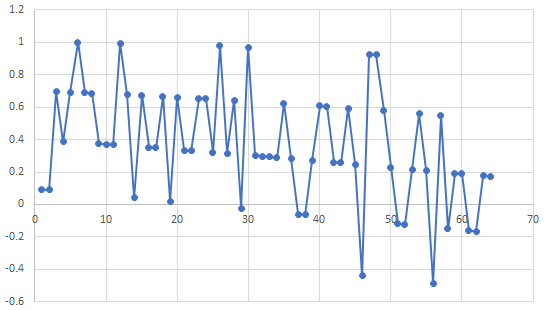
\includegraphics[width=\textwidth]{q8/q8_graph_1.png}
            \caption{graph of estimator 1 against $\frac{k\pi}{2^7}$}
        \end{minipage}
        \hfill
        \begin{minipage}[b]{0.5\linewidth}
            \centering
            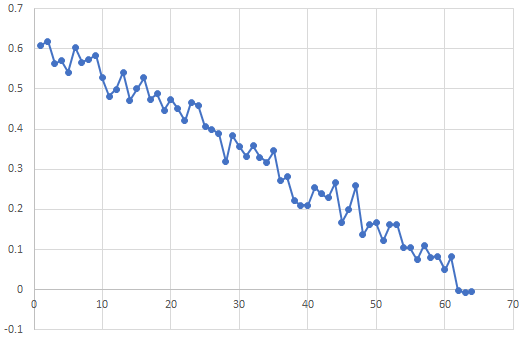
\includegraphics[width=\textwidth]{q8/q8_graph_2.png}
            \caption{graph of estimator 2 against $\frac{k\pi}{2^7}$}
        \end{minipage}
\end{figure}
\noindent
The estimate with level size $N_l=5$ (estimator 1) exhibits much greater variability than the estimator with level size $N_l=2^{L-l}$ (estimator 2).\\
This is evident as we can seen that estimator 2 demonstrates a consistent pattern decreasing from around 0.61 when $k=\frac{\pi}{2^7}$ to around 0 when $k=\frac{2^6\pi}{2^7}$, which matches what should happen analytically as the $\theta$ value increases.\\
Whereas although a gradual decreasing pattern is demonstrated by estimator 1, it is accompanied by fluctuations of large amplitudes, deviating around 0.2 from the line of best fit.\\
This is due to the insufficient number of samples used at low levels for estimator 1, as lower levels carries a greater impact on the overall value. 


\subsection*{Question 9}
$\hat{\mu}N_{1:L}\triangleq\sum_{l=0}^L[\frac{1}{N_l}\sum^{N_l}_{i=1}Y^i_l]$\\
For a MLMC estimator with  truncation level $L$ and level sizes ${N_l}^L_{l=0}$,
\begin{flalign*}
\bm{MSE}(\hat{\mu}N_{1:L},\mu)&=(\bm{E}[\hat{\mu}N_{1:L}]-\mu)^2+\bm{Var}(\hat{\mu}N_{1:L})&\\
&=(\sum\bm{E}[Y_l]-\mu)^2+\sum_{l=0}^L\bm{Var}(\frac{1}{N_l}\sum^{N_l}_{i=1}Y^i_l)&\\
&\leq (\frac{3A_1}{10\times 2^{L}})^2+\sum_{l=0}^L[\frac{1}{N_l}\bm{Var}(Y_l)]\qquad\qquad\text{using results from question 7}&\\
&\leq \frac{9A_1^2}{100\times 4^{L}} + \frac{A_2}{N_0}+A_4\sum_{l=1}^L\frac{h^2_{l-1}}{N_l}\qquad\qquad\text{using fact 2 and 4}&\\
&\underline{=\frac{9A_1^2}{100\times 4^{L}} + \frac{A_2}{N_0}+\frac{A_4}{25}\sum_{l=1}^L\frac{4^{-l}}{N_l}}
\end{flalign*}


\subsection*{Question 10}
We take the computational budget to be some constant $C$. We treat the $N_l$ as continuous variables, and $L=\infty$.\\
We see that $\frac{9A_1^2}{100\times 4^{L}}\rightarrow0$, so we need to minimise $F(x)=\frac{A_2}{N_0}+\frac{A_4}{25}\sum_{l=1}^L\frac{4^{-l}}{N_l}$, where $x=(N_0,N_1,N_2,\dots)$.\\
The constraint is $G(x)=\sum^\infty_{l=0}N_lC_l=C$, where $C_l$ is the constant cost of generating a sample of $Y_l$.\\
So applying a Lagrange multiplier, 
\[H(x,\lambda)=(A_2N_0^{-1}+\lambda N_0C_0)+\sum^\infty_{l=1}[\frac{A_4}{25}N_l^{-1}4^{-l}+\lambda N_lC_l]-\lambda C\]
\begin{flalign*}
&\frac{\delta H}{\delta N_0}= \lambda C_0 - A_2 N_0^{-2} \qquad\qquad\quad \frac{\delta H}{\delta N_l}_{|l\neq0} =\lambda C_l - \frac{A_4 4^{-l}}{25}N_l^{-2} \qquad\qquad\quad \frac{\delta H}{\delta \lambda}=\sum^{\infty}_{l=0}N_lC_l -C &\\
\Longrightarrow \quad&N_0=\sqrt{\frac{A_2}{C_0\lambda}}\qquad\qquad\quad   N_{l|l\neq0}=\sqrt{\frac{A_4}{25\lambda4^lC_l}}&\\
\intertext{thus, setting $\frac{\delta H}{\delta \lambda}=0$, we get}
&\sqrt{\frac{1}{\lambda}}(\sqrt{A_2C_0}+\sum_{l\geq1}\sqrt{\frac{A_4C_l}{25\cdot4^l}})=C\qquad \Longrightarrow \qquad \sqrt{\frac{1}{\lambda}}=\frac{C}{\sqrt{A_2C_0}+\sum_{l\geq1}\sqrt{\frac{A_4C_l}{25\cdot4^l}}}&\\
\end{flalign*}
By subbing in $C_0=10A_3T$ and $C_l=10A_3T(2^l+2^{l-1})$, we may simplify the RHS of the above expression to
\begin{flalign*}
\sqrt{\frac{1}{\lambda}}&=\frac{C}{\sqrt{10TA_2A_3}+\sum_{l=1}^\infty \sqrt{\frac{30A_3A_4T\cdot2^{l-1}}{25\cdot4^l}}}&\\
&=\frac{C}{\sqrt{10TA_2A_3}+\sqrt{\frac{3A_3A_4T}{5}}\sum_{l=1}^\infty2^{-\frac{l}{2}}}&\\
&=\frac{C}{\sqrt{10TA_2A_3}+\sqrt{\frac{3A_3A_4T}{5}}\cdot (1+\sqrt{2})}
\end{flalign*}
Therefore,
\begin{flalign*}
N_0&=\sqrt{\frac{A_2}{10A_3T}}\cdot \frac{C}{\sqrt{10TA_2A_3}+\sqrt{\frac{3A_3A_4T}{5}}\cdot (1+\sqrt{2})}&\\
&=\underline{\frac{C\sqrt{A_2}}{A_3T[10\sqrt{A_2}+(1+\sqrt{2})\sqrt{6A_4}]}}&\\
N_{l|l\neq0}&=\sqrt{\frac{A_4}{750A_3T\cdot2^{3l-1}}}\cdot\frac{C}{\sqrt{10TA_2A_3}+\sqrt{\frac{3A_3A_4T}{5}}\cdot (1+\sqrt{2})}&\\
&=\underline{\frac{C\sqrt{A_4}}{A_3T\cdot2^{\frac{3l-1}{2}}[50\sqrt{3A_2}+(30+15\sqrt{2})\sqrt{A_4}]}}
\end{flalign*}


\subsection*{Question 11}
From results of question 10, we see that for optimal MSE, $N_{l|l\neq0}= k\cdot C\cdot 2^{\frac{-3l}{2}}$, thus if the current truncation level is $L$, then $\lfloor N_L\rfloor=1$ and $\lfloor N_{L+1}\rfloor=0$. \\
So to increase $L$ by 1, we must increase $C$ to $2^{\frac{3}{2}}\cdot C$. This is the same as saying \underline{$C\propto 2^{\frac{3L}{2}}$}.\\
\begin{flalign*}
\bm{MSE}(\hat{\mu}N_{1:L},\mu)&\leq\frac{9A_1^2}{100\times 4^{L}} + \frac{A_2}{N_0}+\frac{A_4}{25}\sum_{l=1}^L\frac{4^{-l}}{N_l}&\\
&=m\cdot 4^{-L} + n\cdot C^{-1} + p \cdot \sum_{l=1}^L 4^{-l}C^{-1}2^{\frac{3l}{2}}  \qquad\qquad\text{where m,n,p are constants}&\\
&=m\cdot 4^{-L} + n\cdot C^{-1} + p \cdot C^{-1} \sum_{l=1}^L 2^{-\frac{l}{2}}&\\
\intertext{with some rearrangements, we get $4^{-L}\propto C^{\frac{-4}{3}}$, and $\sum_{l=1}^L 2^{-\frac{l}{2}} = (1+\sqrt{2})(1-2^{\frac{-L}{2}})$. We can find further that $2^{\frac{-L}{2}}\propto C^{\frac{-1}{3}}$. Therefore,}
\text{MSE upper bound} & \propto C^{\frac{-4}{3}} + C^{-1} + C^{-1}\cdot (1-C^{\frac{-1}{3}})&\\
&\underline{\propto C^{-1}} \qquad\qquad\text{(as $C^{-1}$ is the dominant power)}
\end{flalign*}
This is better than the MC estimator described in Question 6, since the $\bm{MSE}_{MLMC}\propto C^{-1}$ whereas $\bm{MSE}_{MC}\propto C^{-\frac{2}{3}}$.\\
Which means for the same increase in computational cost C, the upper bound for the MSE of the MLMC estimator will decrease more than the upper bound for the MSE of the MC estimator.\\
Hence the MLMC estimator is more accurate than the MC estimator.


\section*{Application to Double-Well Loss Function}

\subsection*{Question 12}
We suppose $h>0$ small enough and $T\in\bm{N}$ large enough, such that $min{|m_1(\theta)-X^h_T|,|m_2(\theta)-X^h_T|}\approx 0$ for any initial point $x_0\in [-1,1]$. \\
Therefore, we know $\lim_{T\to\infty}X^h_T$ converges to either $m_1(\theta)$ or $m_2(\theta)$.\\
Hence, 
\begin{align}
p_1m_1(\theta)+p_2m_2(\theta)=\mu\\
p_1+p_2=1    
\end{align}
Rearranging (2) to get $p_1=1-p_2$ and sub into (1) to get 
\begin{flalign*}
(m_1(\theta)-m_2(\theta))p_1&=\mu-m_2(\theta)\\
p_1&=\frac{m_2(\theta)-\mu}{m_2(\theta)-m_1(\theta)}\\
\intertext{and hence,}
p_2&=\frac{\mu-m_1(\theta)}{m_2(\theta)-m_1(\theta)}
\end{flalign*}


\subsection*{Question 13}
The code used to produce the estimator with level size $N_l=2^{L-l}$ is attached in the programs section under the title \emph{'iv) q13\textunderscore probability.m'}\\
We use the formula derived for $N_l$ in question 10 to find the optimal level size. We choose C to be $10^7$ as that provides a reasonable calculation time, and we pick $A_2, A_3$ and $A_4$ all to be 1.\\
The above constants gives a 8-level MLMC estimator.\\
\begin{tabular}{|c|c|}
\hline
level $l$ & level size\\
\hline
0     & 62839\\
1    & 1282\\
2     & 453\\
3     & 160\\
4    & 56\\
5     & 20\\
6    & 7\\
7   &  2\\
\hline
\end{tabular}\\\\\\
Below is the graph of $p_1$ and $p_2$ as k varies.
\begin{figure}[h]
    \centering
    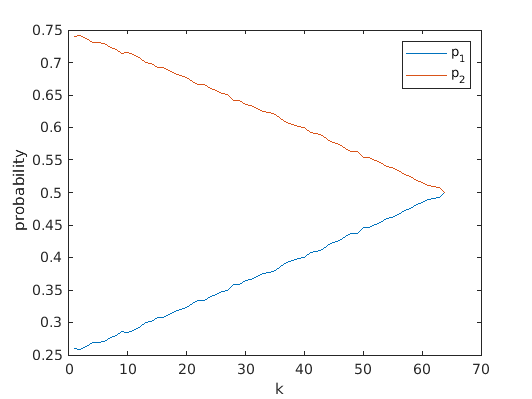
\includegraphics[width=0.5\textwidth]{q13/q13.png}
    \caption{graph of $p_1$ and $p_2$ against k}
\end{figure}
\noindent
We can see that $p_1$ increases consistently from about 0.25 to 0.5, which is what we'd expect, and the smoothness of the increase shows the the MLMC method we employed is accurate and has a small MSE.\\
\newpage
\noindent
To find out for which values of $\theta$ does the outcome move fast, we first calculate it analytically.
\begin{flalign*}
p_1 &=  \frac{\cos(\frac{x+4\pi}{3}) - (-1)}{2}&\\
& =\frac{1}{2}+\frac{1}{2}\cos(\frac{x+4\pi}{3})&\\
\frac{dp_1}{dx} &= -\frac{1}{6}\sin(\frac{x+4\pi}{3})&
\end{flalign*}
In this question, $x$ takes values in $(0,\frac{\pi}{2})$, hence $\frac{dp_1}{dx}$ takes value between $-\frac{1}{6}\sin(\frac{4\pi}{3})$ and $-\frac{1}{6}\sin(\frac{3\pi}{2})$.\\
Therefore, from property of the $sin$ function, we know that $p_1$ increase faster at larger values of $\theta$, and increase slower at smaller values of $\theta$.
And hence by symmetry, $p_2$ decreases faster at large values of $\theta$.\\\\
Then we can plot out the difference in outcome between adjacent values of $k$ to confirm the trend. The code used to do that is as below.
 \begin{lstlisting}
% for plotting the difference between adjacent points
for i = 1:63
    difference(i) = results_p1(z+1) - results_p1(z);
end
plot(difference)
\end{lstlisting}
\begin{figure}[h]
        \centering
        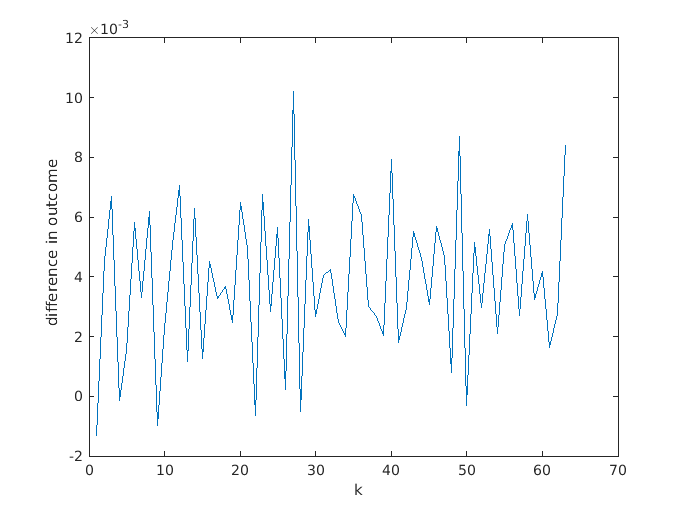
\includegraphics[width=250pt]{q13/q13_difference.png}
        \caption{graph of difference between adjacent values of k}
\end{figure}
We can see from the graph that as k increases, there is a slight increase in the difference in the outcome between adjacent values of k, thus our estimates confirms the analytic results. 


\newpage
\section*{Tables}
\subsection*{i) q8 estimator results}
\begin{tabular}{c|c}

\begin{tabular}{|c|c|c|}
\hline
$k\times\frac{\pi}{2^7}$ & $\mu N_{1:L}$ with $N_l=5$ & $\mu N_{1:L}$ with $N_l=2^{L-l}$ \\ 
\hline 
1 & 0.090284 & 0.60831\\ 
2 & 0.089218 & 0.61826\\ 
3 & 0.69497 & 0.56301\\ 
4 & 0.3879 & 0.57152\\ 
5 & 0.69221 & 0.54166 \\ 
6 & 0.9988 & 0.60401\\ 
7 & 0.68891 & 0.56638 \\ 
8 & 0.68716 & 0.57312\\ 
9 & 0.37343 & 0.58304  \\ 
10 & 0.37036 & 0.52724\\ 
11 & 0.36725 & 0.48175 \\ 
12 & 0.99519 & 0.49909\\ 
13 & 0.67766 & 0.54127\\ 
14 & 0.03996 & 0.47201\\ 
15 & 0.67353 & 0.50036\\ 
16 & 0.35136 & 0.52732\\ 
17 & 0.34811 &0.47449\\ 
18 & 0.66701 &0.48736\\ 
19 & 0.018348 &0.44665\\ 
20 & 0.66244 &0.47374\\ 
21 & 0.33489 &0.45017\\ 
22 & 0.33153 &0.42007\\ 
23 & 0.65524 &0.46646\\ 
24 & 0.65276 &0.45863\\ 
25 & 0.3213 &0.40578\\ 
26 & 0.97746 & 0.39934\\ 
27 & 0.31438 &0.38801\\ 
28 & 0.64238& 0.31833\\ 
29 & -0.02493 &0.38461\\ 
30 & 0.97003 &0.35686\\ 
31 & 0.30029 &0.33224\\ 
32 & 0.29671& 0.35814\\ 
\hline
\end{tabular}
\begin{tabular}{|c|c|c|}
\hline
$k\times\frac{\pi}{2^7}$ & $\mu N_{1:L}$ with $N_l=5$ & $\mu N_{1:L}$ with $N_l=2^{L-l}$ \\ 
\hline
33 & 0.29312& 0.33012\\ 
34 & 0.2895& 0.31674\\ 
35 & 0.62258 &0.34604\\ 
36 & 0.28222& 0.27168\\ 
37 & -0.059446 &0.28119\\ 
38 & -0.063746& 0.22129\\ 
39 & 0.27115& 0.21086\\ 
40 & 0.60718 &0.21035\\ 
41 & 0.60397 &0.25471\\ 
42 & 0.25992 &0.23928\\ 
43 & 0.25614 &0.2288\\ 
44 & 0.59412& 0.26669\\ 
45 & 0.24853 &0.16765\\ 
46 & -0.44063& 0.20052\\ 
47 & 0.92698& 0.25861\\ 
48 & 0.92388 &0.13737\\ 
49 & 0.57691 &0.16193\\ 
50 & 0.22921 &0.16637\\ 
51 & -0.11915 &0.12204\\ 
52 & -0.12336 &0.16179\\ 
53 & 0.21744 &0.16286\\ 
54 & 0.55874 &0.10492\\ 
55 & 0.20952 &0.10426\\ 
56 & -0.4858 &0.074897\\ 
57 & 0.54738 &0.11136\\ 
58 & -0.14846 &0.080285\\ 
59 & 0.19351 &0.082979\\ 
60 & 0.18947 &0.050171\\ 
61 & -0.16088 &0.081599\\ 
62 & -0.165& -0.0019665\\ 
63 & 0.17729 &-0.00600578\\ 
64 & 0.17321 &-0.0033829\\ 
\hline
\end{tabular}
\end{tabular}

\newpage
\section*{Programs}
\bigskip
\subsection*{i) q2\textunderscore gradient\textunderscore descent.m}
\lstdefinestyle{myCustomMatlabStyle}{
  language=Matlab,
  stepnumber=1,
  numbersep=10pt,
  tabsize=4,
  showspaces=false,
  showstringspaces=false
}
\lstset{basicstyle=\footnotesize,style=myCustomMatlabStyle}
\begin{lstlisting}
theta = pi/6;
h = 0.01;
grad_f = @(x) 4*x^3-3*x-cos(theta);
X = zeros(101,1);   % to store the final outcome
for i = 1:101
    x_a = (i-51)/50;        % set initial value
    for j = 1:1000
        x_b = x_a - h*grad_f(x_a);      % alg iteration
        x_a = x_b;
    end
    X(i) = x_b;
end
T=table([-1:0.02:1].',X);
disp(T)
\end{lstlisting}

\bigskip\bigskip\bigskip
\subsection*{ii) q4\textunderscore monte\textunderscore carlo\textunderscore gradient\textunderscore descent.m}
\lstdefinestyle{myCustomMatlabStyle}{
  language=Matlab,
  stepnumber=1,
  numbersep=10pt,
  tabsize=4,
  showspaces=false,
  showstringspaces=false
}
\lstset{basicstyle=\footnotesize,style=myCustomMatlabStyle}
\begin{lstlisting}
theta = pi/4;
grad_f = @(x) 4*x^3-3*x-cos(theta);
T = 10;
mu_estimator = zeros(11,1);     % store values of mu_h
var_estimator = zeros(11,1);      % store values of variance of X
for k = 0:10
    h = 0.1*2^(-k);
    iter_required = T/h;        % number of iterations per sample
    N = 2^(20-k);           % number of samples used
    temp_results=zeros(N,1);        % stores outcome of samples
    for n = 1:N
        x_a = 2*rand -1;         % random number in [-1,1]
        for i = 1:iter_required
            x_b = x_a - h*grad_f(x_a);      % alg iteration
            x_a = x_b;
        end
        temp_results(n) = x_a;
    end
    mu_estimator(k+1) = mean(temp_results);     % find the expectation using averages
    var_estimator(k+1) = var(temp_results);
end
table([0:10].',mu_estimator,var_estimator)
\end{lstlisting}

\newpage
\subsection*{iii) q8\textunderscore MLMC.m}
\lstdefinestyle{myCustomMatlabStyle}{
  language=Matlab,
  stepnumber=1,
  numbersep=10pt,
  tabsize=4,
  showspaces=false,
  showstringspaces=false
}
\lstset{basicstyle=\footnotesize,style=myCustomMatlabStyle}
\begin{lstlisting}
format long
T = 10;
L = 10;         %fixed truncation level
results=zeros(2^6,1);       
for k = 1:2^6
    theta = k*pi/2^7;
    grad_f = @(x) 4*x^3-3*x-cos(theta); 
    mu_estimator = 0;       %stores value of mu
% below is used to calculate Y_0    
    h_0 = 0.1*2^0;
    iter_required = T/h_0;
    N = 2^L;       % change to 5 for Q8 part i)
    Y = zeros(1,N);
    for i = 1:N
        x_a = 2*rand -1;         % random number in [-1,1]
        for j = 1:iter_required
            x_b = x_a - h_0*grad_f(x_a);      % alg iteration
            x_a = x_b;
        end
        Y(i) = x_a;
    end
    mu_estimator = mu_estimator + mean(Y);
% below is used to calculate Y_l, l not 0
    for l = 1:10
        N = 2^(L-l);        % change to 5 for Q8 part i)
        Y = zeros(1,N);        
        h_1 = 0.1*2^(-l);
        h_2 = 0.1*2^(-l+1);
        iter_h_1 = T/h_1;        % number of iterations for h_l
        iter_h_2 = T/h_2;        % number of iterations for h_(l-1)
        for i = 1:N
            x_0 = 2*rand -1;         
         
            x_a = x_0;      %copy of initial point for X_(h_l)
            for j = 1:iter_h_1
                x_b = x_a - h_1*grad_f(x_a);      
                x_a = x_b;
            end
         
            x_c = x_0;      %copy of initial point for X_(h_(l-1))
            for j = 1:iter_h_2
                x_d = x_c - h_2*grad_f(x_c);      
                x_c = x_d;
            end
            Y(i) = x_a - x_c;
        end
        mu_estimator = mu_estimator + mean(Y);     % sum up the mean of Y_l
    end
    results(k) = mu_estimator;
end
T=table(1:2^6,results);
disp(T)
\end{lstlisting}
\newpage
\subsection*{iv) q13\textunderscore probability.m}
\lstdefinestyle{myCustomMatlabStyle}{
  language=Matlab,
  stepnumber=1,
  numbersep=10pt,
  tabsize=4,
  showspaces=false,
  showstringspaces=false
}
\lstset{basicstyle=\footnotesize,style=myCustomMatlabStyle}
\begin{lstlisting}
format long
A_2 = 1;        % setting constants
A_3 = 1;
A_4 = 1;
C = 10^7;
T = 10;
N(1) = (C*sqrt(A_2))/(A_3*T*(10*sqrt(A_2)+(1+sqrt(2))*sqrt(6*A_4)));
l=1;
while floor(N(l)) > 0       % calculates level sizes and number of levels
    l = l+1;
    N(l) = (C*sqrt(A_4))/((A_3*T*2^((3*l-1)/2))*(50*sqrt(3*A_2) ...
        + (30+15*sqrt(2))*sqrt(A_4)));    
end
N = floor(N);
L = numel(N)-2;     % highest level
results_p1 = zeros(1,2^6);      %stores value of p1
results_p2 = zeros(1,2^6);      %stores value of p2

for k = 1:2^6
    theta = k*pi/2^7;
    grad_f = @(x) 4*x^3-3*x-cos(theta);
    m1 = cos((theta+2*pi)/3);
    m2 = cos(theta/3);
    mu_estimator = 0;       %stores value of mu
% below is used to calculate Y_0    
    h_0 = 0.1*2^0;
    iter_required = T/h_0;
    n_0 = N(1);       
    Y = zeros(1,n_0);
    for i = 1:n_0
        x_a = 2*rand -1;         % random number in [-1,1]
        for j = 1:iter_required
            x_b = x_a - h_0*grad_f(x_a);      % alg iteration
            x_a = x_b;
        end
        Y(i) = x_a;
    end
    mu_estimator = mu_estimator + mean(Y);
% below is used to calculate Y_l, l not 0
    for l = 1:L
        n_l = N(l+1);        
        Y = zeros(1,n_l);        
        h_1 = 0.1*2^(-l);
        h_2 = 0.1*2^(-l+1);
        iter_h_1 = T/h_1;        % number of iterations for h_l
        iter_h_2 = T/h_2;        % number of iterations for h_(l-1)
        for i = 1:n_l
            x_0 = 2*rand -1;         
         
            x_a = x_0;      %copy of initial point for X_(h_l)
            for j = 1:iter_h_1
                x_b = x_a - h_1*grad_f(x_a);      
                x_a = x_b;
            end
            x_c = x_0;      %copy of initial point for X_(h_(l-1))
            for j = 1:iter_h_2
                x_d = x_c - h_2*grad_f(x_c);      
                x_c = x_d;
            end
            Y(i) = x_a - x_c;
        end
        mu_estimator = mu_estimator + mean(Y);     % sum up the mean of Y_l
    end
    results_p1(k) = (m2-mu_estimator)/(m2-m1);      % calculates p1
    results_p2(k) = (mu_estimator-m1)/(m2-m1);      % calculates p2
end
%below plots the graph
X = linspace(1,64,64);
plot(X,results_p1,"DisplayName","p_1")
hold on
plot(X,results_p2,"DisplayName","p_2")
hold off
legend
\end{lstlisting}

\end{document}